%!TEX root = ./paper.tex

\section*{Appendix}

\begin{figure}[h]
  \centering 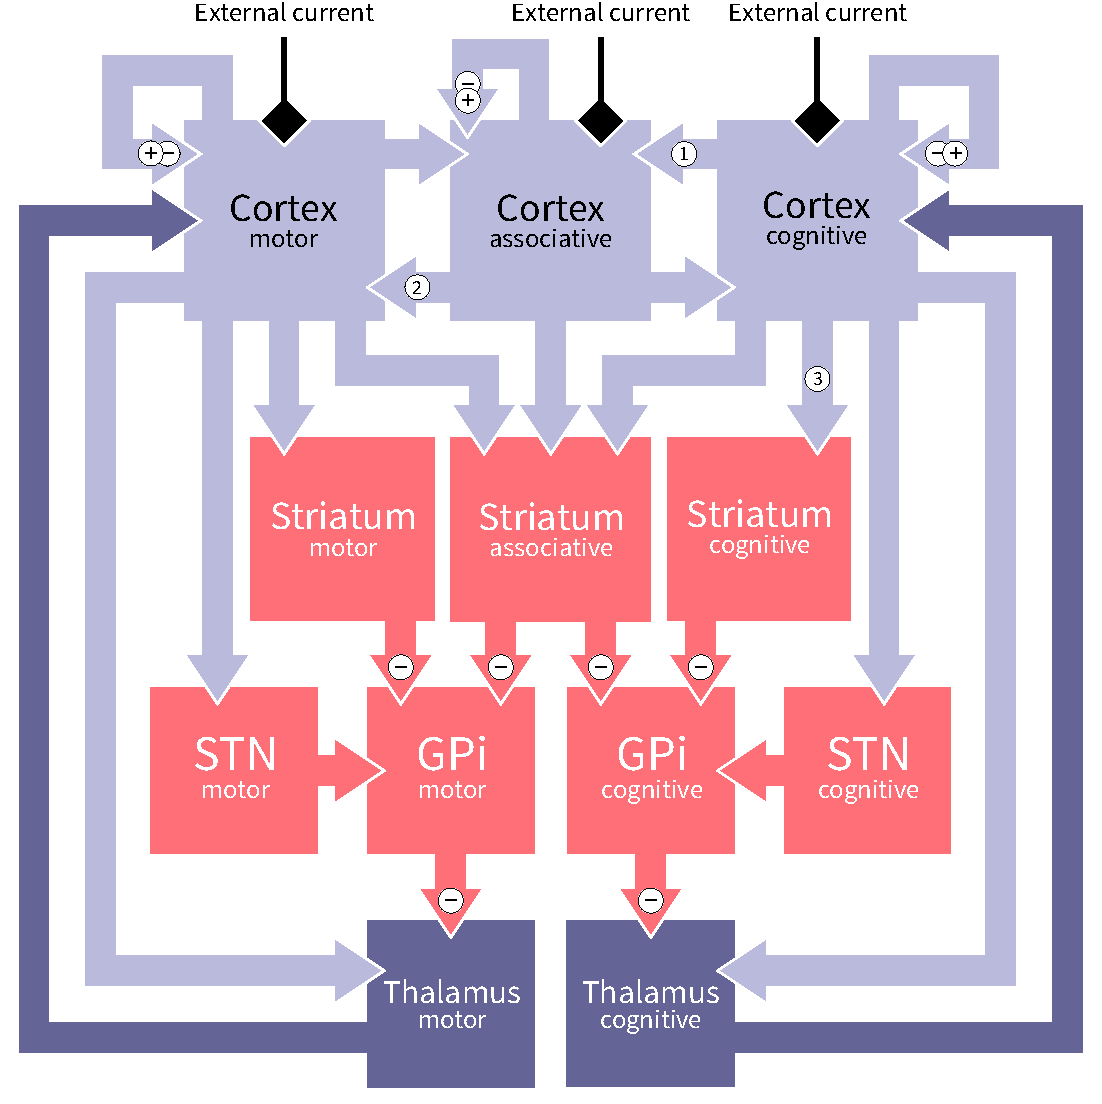
\includegraphics[width=0.5\textwidth]{architecture}
  \caption{Architecture of the model}
  \label{fig:architecture}
\end{figure}



\begin{figure}[h]
        \centering
        \begin{subfigure}[b]{0.3\textwidth}
                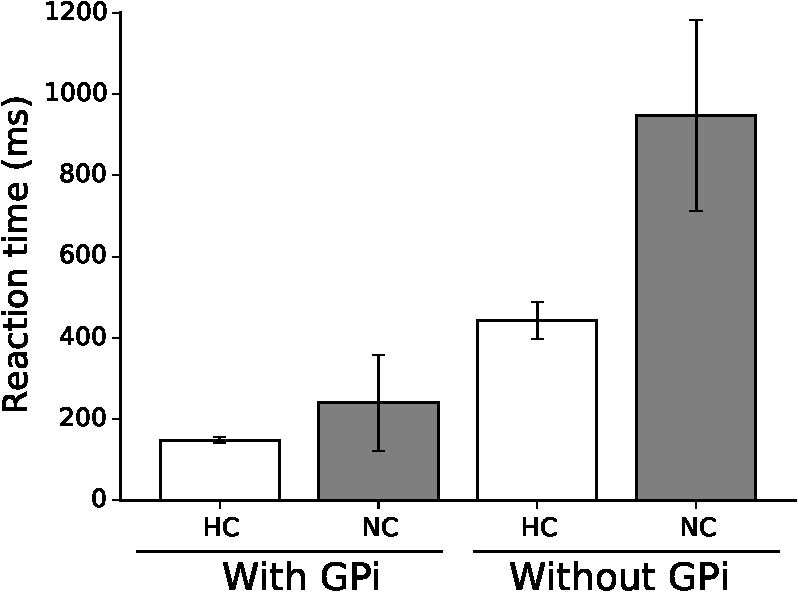
\includegraphics[width=\textwidth]{RTresults}
                \caption{RTresults of the model}
                \label{fig:RTresults}
        \end{subfigure}
        ~ %add desired spacing between images, e. g. ~, \quad, \qquad, \hfill etc.
          %(or a blank line to force the subfigure onto a new line)
          
        \begin{subfigure}[b]{0.5\textwidth}
                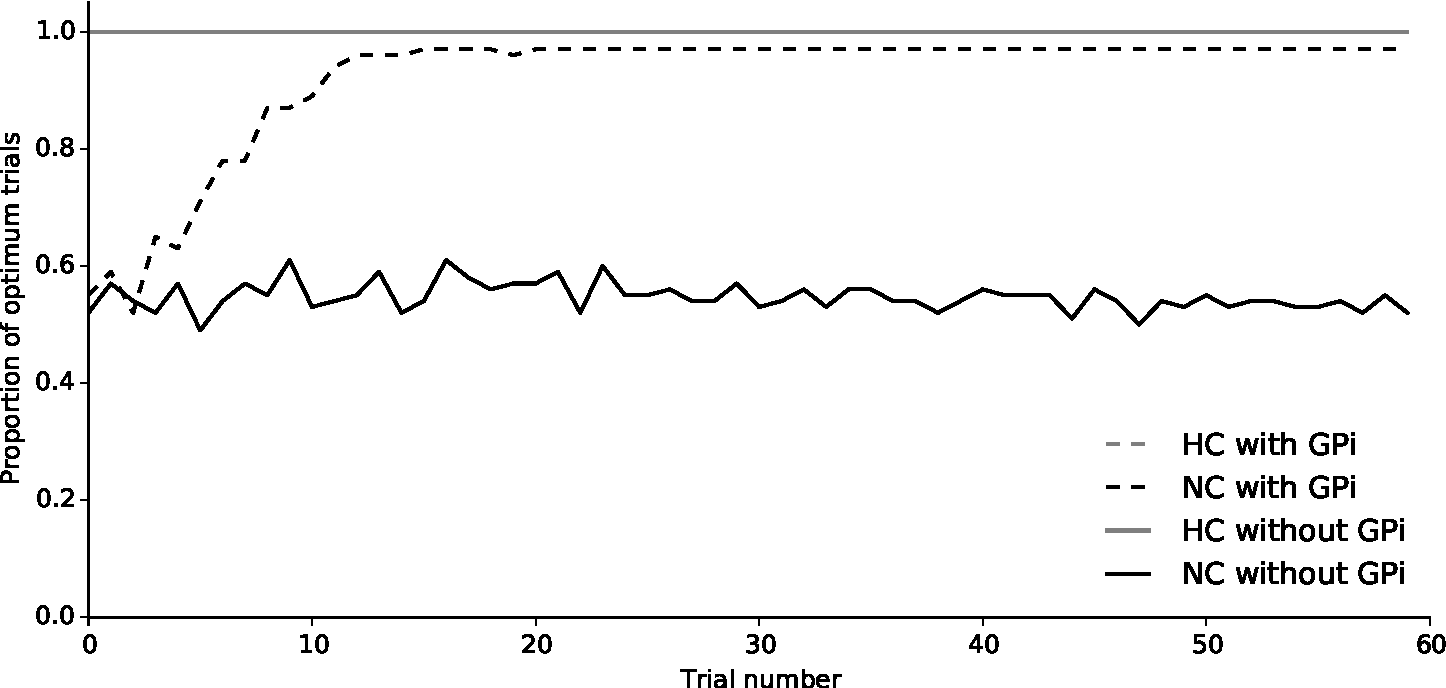
\includegraphics[width=\textwidth]{Performances}
                \caption{Performances of the model}
                \label{fig:Performances}
        \end{subfigure}
        \caption{Results of the model}\label{fig:Results}
\end{figure}

